\documentclass[letterpaper,english,11pt]{article}
\usepackage{%
	amsfonts,%
	amsmath,%	
	amssymb,%
	amsthm,%
	babel,%
	bbm,%
	%biblatex,%
	caption,%
	centernot,%
	color,%
	enumerate,%
	%enumitem,%
	epsfig,%
	epstopdf,%
	etex,%
	fancybox,%
	framed,%
	fullpage,%
	%geometry,%
	graphicx,%
	hyperref,%
	latexsym,%
	mathptmx,%
	mathtools,%
	multicol,%
	pgf,%
	pgfplots,%
	pgfplotstable,%
	pgfpages,%
	proof,%
	psfrag,%
	%subfigure,%	
	tikz,%
	times,%
	ulem,%
	url,%
	xcolor,%
	mathpazo
}

\definecolor{shadecolor}{gray}{.95}%{rgb}{1,0,0}
\usepackage[margin=1in,top=0.75in]{geometry}
\usepackage[mathscr]{eucal}
\usepgflibrary{shapes}
\usepgfplotslibrary{fillbetween}
\usetikzlibrary{%
  arrows,%
  backgrounds,%
  chains,%
  decorations.pathmorphing,% /pgf/decoration/random steps | erste Graphik
  decorations.text,% 
  matrix,%
  positioning,% wg. " of "
  fit,%
  patterns,%
  petri,%
  plotmarks,%
  scopes,%
  shadows,%
  shapes.misc,% wg. rounded rectangle
  shapes.arrows,%
  shapes.callouts,%
  shapes%
}

%\pgfplotsset{compat=newest} %<------ Here
\pgfplotsset{compat=1.11} %<------ Or use this one

\theoremstyle{plain}
\newtheorem{thm}{Theorem}[section]
\newtheorem{lem}[thm]{Lemma}
\newtheorem{prop}[thm]{Proposition}
\newtheorem{cor}[thm]{Corollary}
\newtheorem{clm}[thm]{Claim}

\theoremstyle{definition}
\newtheorem{axiom}[thm]{Axiom}
\newtheorem{defn}[thm]{Definition}
\newtheorem{conj}[thm]{Conjecture}
\newtheorem{exmp}[thm]{Example}
\newtheorem{exerc}[thm]{Exercise}
\newtheorem{assum}[thm]{Assumptions}

\theoremstyle{remark}
\newtheorem{rem}[thm]{Remark}
\newtheorem{note}[thm]{Note}

\newcommand{\Cov}{\operatorname{Cov}}
%\newcommand{\det}{\operatorname{det}}
\newcommand{\Real}{\mathbb{R}}
\newcommand{\tr}{\operatorname{tr}}
%\newcommand{\Var}{\operatorname{Var}}

\DeclareMathOperator{\sign}{sign}
%\renewcommand{\proof}[1]{\begin{proof}#1\end{proof}}
\newcommand{\EQ}[1]{\begin{equation*}#1\end{equation*}}
\newcommand{\EQN}[1]{\begin{equation}#1\end{equation}}
\newcommand{\eq}[1]{\begin{align*}#1\end{align*}}
\newcommand{\meq}[2]{\begin{xalignat*}{#1}#2\end{xalignat*}}
\newcommand{\norm}[1]{\left\lVert#1\right\rVert}
\newcommand{\abs}[1]{\left\lvert#1\right\rvert}
\newcommand{\expect}[1]{\mathbb{E}\left[{#1}\right]}
\newcommand{\prob}[1]{\mathbb{P}\left[{#1}\right]}
\newcommand{\given}{\; \big\vert \;} 
\newcommand{\set}[1]{\left\{#1\right\}} 
\newcommand{\indicator}[1]{\mathbb{1}_{\set{#1}}} 
\newcommand{\inner}[1]{\left\langle#1\right\rangle}
\newcommand{\red}[1]{\textcolor{red}{#1}} 
\newcommand{\E}[1]{\mathbb{E}\left[#1\right]}
\newcommand{\Var}[1]{\operatorname{Var}\left[#1\right]}

\newcommand{\D}{\mathbb{D}}
%\newcommand{\E}{\mathbb{E}}
\newcommand{\N}{\mathbb{N}}
\renewcommand{\P}{\mathbb{P}}
\newcommand{\Q}{\mathbb{Q}}
\newcommand{\R}{\mathbb{R}}
\newcommand{\Z}{\mathbb{Z}}

\newcommand{\bU}{\mathbf{1}}
\newcommand{\bx}{\mathbf{x}}

\newcommand{\cB}{\mathcal{B}}
\newcommand{\cC}{\mathcal{C}}
\newcommand{\cD}{\mathcal{D}}
\newcommand{\cF}{\mathcal{F}}
\newcommand{\cG}{\mathcal{G}}
\newcommand{\cH}{\mathcal{H}}
\newcommand{\cO}{\mathcal{O}}
\newcommand{\cT}{\mathcal{T}}
\newcommand{\cX}{\mathcal{X}}
\newcommand{\cY}{\mathcal{Y}}

\newcommand{\sA}{\mathscr{A}}
\newcommand{\sB}{\mathscr{B}}
\newcommand{\sC}{\mathscr{C}}
\newcommand{\sD}{\mathscr{D}}
\newcommand{\sE}{\mathscr{E}}
\newcommand{\sF}{\mathscr{F}}
\newcommand{\sG}{\mathscr{G}}
\newcommand{\sH}{\mathscr{H}}
\newcommand{\sL}{\mathscr{L}}
\newcommand{\dO}{\mathscr{O}}
\newcommand{\sS}{\mathscr{S}}
\newcommand{\sT}{\mathscr{T}}
\newcommand{\sX}{\mathscr{X}}
\newcommand{\sY}{\mathscr{Y}}
\newcommand{\sZ}{\mathscr{Z}}

% Debug
\newcommand{\todo}[1]{\begin{color}{blue}{{\bf~[TODO:~#1]}}\end{color}}

% a few handy macros

\renewcommand{\le}{\leqslant}
\renewcommand{\ge}{\geqslant}
\newcommand\matlab{{\sc matlab}}
\newcommand{\goto}{\rightarrow}
\newcommand{\bigo}{{\mathcal O}}
%\newcommand{\half}{\frac{1}{2}}
%\newcommand\implies{\quad\Longrightarrow\quad}
\newcommand\reals{{{\rm l} \kern -.15em {\rm R} }}
\newcommand\complex{{\raisebox{.043ex}{\rule{0.07em}{1.56ex}} \hskip -.35em {\rm C}}}


% macros for matrices/vectors:

% matrix environment for vectors or matrices where elements are centered
\newenvironment{mat}{\left[\begin{array}{ccccccccccccccc}}{\end{array}\right]}
\newcommand\bcm{\begin{mat}}
\newcommand\ecm{\end{mat}}

% matrix environment for vectors or matrices where elements are right justifvied
\newenvironment{rmat}{\left[\begin{array}{rrrrrrrrrrrrr}}{\end{array}\right]}
\newcommand\brm{\begin{rmat}}
\newcommand\erm{\end{rmat}}

% for left brace and a set of choices
%\newenvironment{choices}{\left\{ \begin{array}{ll}}{\end{array}\right.}
\newcommand\when{&\text{if~}}
\newcommand\otherwise{&\text{otherwise}}
% sample usage:
%  \delta_{ij} = \begin{choices} 1 \when i=j, \\ 0 \otherwise \end{choices}


% for labeling and referencing equations:
\newcommand{\eql}{\begin{equation}\label}
\newcommand{\eqn}[1]{(\ref{#1})}
% can then do
%  \eql{eqnlabel}
%  ...
%  \end{equation}
% and refer to it as equation \eqn{eqnlabel}.  


% some useful macros for finite difference methods:
\newcommand\unp{U^{n+1}}
\newcommand\unm{U^{n-1}}

% for chemical reactions:
\newcommand{\react}[1]{\stackrel{K_{#1}}{\rightarrow}}
\newcommand{\reactb}[2]{\stackrel{K_{#1}}{~\stackrel{\rightleftharpoons}
   {\scriptstyle K_{#2}}}~}


\makeatletter
\def\th@plain{%
  \thm@notefont{}% same as heading font
  \itshape % body font
}
\def\th@definition{%
  \thm@notefont{}% same as heading font
  \normalfont % body font
}
\makeatother
\date{}

\usepackage{algorithm2e}
\usepackage{subfigure}
\usepackage{bm}
%opening
\title{Lecture-29: Study of Opinion Formation using a Modified Vicsek-like Model}
\author{Author: Narayani Vedam}

\begin{document}
\maketitle
\section{Introduction}

 With the wide spread of internet, there is a drastic change in the way opinions are formed. They are increasingly shaped by information diffused through posts on virtual platforms. This impacts the behaviour of individuals and societies. Because of their relevance to social and economic problems, there is a growing interest to understand the underlying dynamics. The aim of this study is to emulate (a) interactions over virtual social platforms, and (b) thereby the coevolution of opinions and the interaction network.

\section{Vicsek Model}

In 1994, inspired by biological interactions, Vicsek proposed a model to study self-ordered motion of particles in a non-equilibrium system. They suggested that the particles be placed uniformly at random ($x_{i}(t)$) with different headings ($\theta_{i}(t)$) in a periodic square box of size $L$.  Each particle is driven by a constant absolute velocity $v$ and at each time-step the particles update their position according to the following update rule, 
\begin{equation}
x_{i}(t+1)= x_{i}(t)+ v_{i}(t)\Delta t,~\text{where}~\Delta t = 1.
 \end{equation}
The velocity is also updated, $v_{i}(t) = v e^{j\theta_{i}(t)}.$ The particles only interact with those within a radius $r$, and update their heading to the respective group average ($\langle \theta(t)\rangle_{r}$), 
\begin{align}
\theta(t+1) &= \langle \theta(t)\rangle_{r} +\Delta \theta,~\text{where} \\
\langle \theta(t)\rangle_{r} &= \arctan \bigg(\frac{\langle\sin(\theta(t))\rangle_{r}}{\langle\cos(\theta(t))\rangle_{r}}\bigg).
\end{align}
In (3), $\Delta \theta$ is a random number chosen with an uniform probability from the interval $[-\frac{\eta}{2},\frac{\eta}{2}]$. Thus, there are three free parameters in the system - $\text{noise}~(\eta),~\text{density}~(\rho),~\text{and}~v$. 

In the limit $v\rightarrow 0$, the particles do not move, and for $v\rightarrow \infty$ the particles become completely mixed up between two updates. Therefore, $0.03<v<0.3$ is chosen for the study. For a fixed velocity, the behavior of the system for different noise and density was simulated. It was observed that at high density and low noise the particles tend to move in the same spontaneously chosen direction. For small densities and noise, the particles tend to form groups moving coherently in random directions. However, at higher noise the particles move randomly with some correlation. 

To study the kinetic phase transition a parameter called the average normalized velocity, 
\begin{equation}
v_{a} = \frac{1}{Nv}|\sum_{i=1}^{N}v_{i}|
\end{equation} was used. This velocity is approximately zero if the direction of motion of individual particles is distributed randomly. However, for a coherently moving phase with ordered direction of velocities, $v_{a}\approx 1$. So, we can consider the average velocity as an order parameter. 

The rule corresponding to aligning spins in a ferromagnetic model is replaced by a rule that aligns direction of motion of particles. Therefore, the Vicsek model that is inherently dynamic and lattice free is a non-equilibrium analog of the ferromagnetic models. This nearest neighbor rule has indicated consensus about the heading, despite the absence of centralized co-ordination and a dynamic neighborhood. This, coupled with the model's simplicity, makes it a popular choice for studying robotic swarms. It has been extensively used for data fusion in sensor networks, collaboration of UAVs, and in explaining the behavior of animal groups
\section{Modified Vicsek-like Model}
We adapt the model in \cite{vicsek1995novel} since the nearest-neighbor rule with dynamic local interactions epitomizes influence spread in networks. We assume that beliefs of members of a social group are analogous to the direction of motion of a particle in space.

Consider $N$ agents, each with a belief $\theta_{i}(t) \in [0,\pi]$. An agent engages with those others, whose beliefs do not deviate from its own by more than a fixed tolerance ($\theta_{T_{i}}$). This is similar to interactions over virtual networks that are oblivious to geographic locations of agents and the distances separating them. The like-minded individuals who influence an agent, constitute its opinion neighborhood,
\begin{equation}
N_{i}(t)~:=~\{~j~:~|\theta_{i}(t)-\theta_{j}(t)|~\leq ~\theta_{T_{i}}\}.
\end{equation}
In Fig. \ref{fig1}, the vectors represent opinions and shaded sectors indicate tolerances. It is clear that the sectors of agents $1$ and $2$ overlap the opinion vectors of $2$ and $1$, respectively. The same can be observed with $2$ and $3$, indicating they are neighbors.
\begin{figure}[t!]	
	\centering
	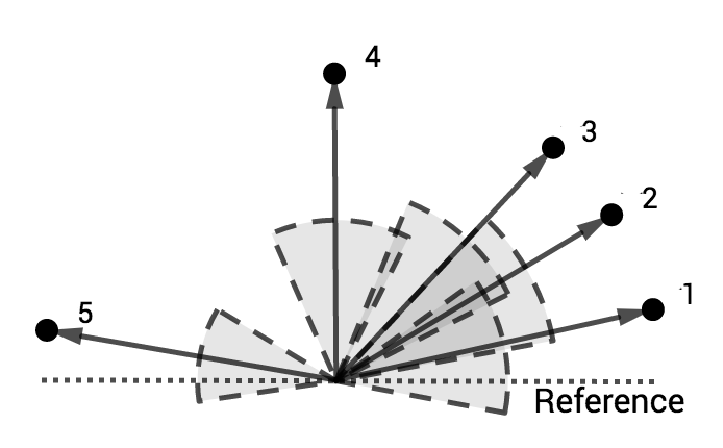
\includegraphics[width=4.5cm]{opinionvectors.eps}
	\vspace{-5pt}
	\caption{Opinion vectors with shaded sectors indicating tolerance ($\theta_{T_{i}}$)}	
	\label{fig1}\vspace{-15pt}
\end{figure}
The agents and their influence can be abstracted using vertices and directed edges of a graph $G(t)= (V,E(t))$. Its vertex set $V$ is invariable and is a collection of $N$ agents. Its edge set $E(t)$ is a collection of all the interactions at time $t$,
\begin{equation}
E(t)~\subseteq~\{~(i,j)~:~j\in~N_{i}(t)~,~\forall i,~i~\neq~j~\}.
\end{equation} 
The directed edge $(i,j)$ is the influence of $i$ on $j$. To illustrate, consider the agents and their tolerance as portrayed in Fig.\ref{fig1}. The corresponding vertex and edge sets are $V=\{1,2,3,4,5\}$ and $E(t)=\{(1,2),(2,1),(2,3),(3,1)\}$, respectively. This is represented in Fig. \ref{fig2a} where there are bidirectional edges between vertex pairs $(1, 2)$ and $(2, 3)$. The beliefs of $4$ and $5$ are different from the rest, and are isolated. Fig. \ref{fig2b} depicts a more realistic scenario, where influences are not reciprocated. It can be observed that 2 influences 1, while 1 does not influence 2. Similarly, 3 influences 2 and not vice versa. 
\begin{figure}[t!]	
	\centering
	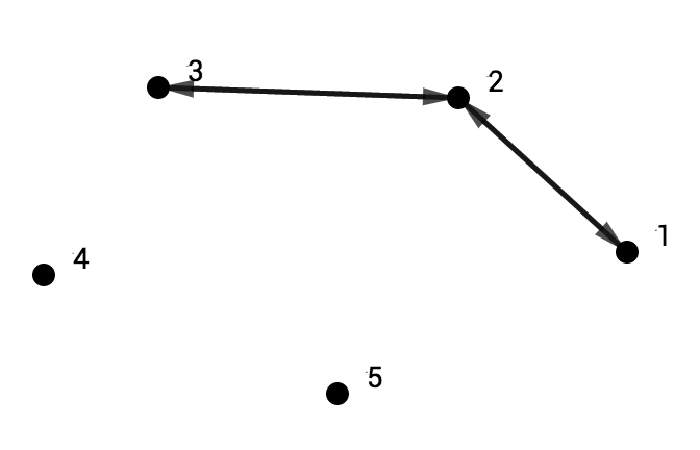
\includegraphics[width=4.5cm]{graph1.eps}
	\vspace{-5pt}
	\caption{Agents and their influence}	
	\label{fig2a}\vspace{-15pt}
\end{figure}

\begin{figure}[t!]	
	\centering
	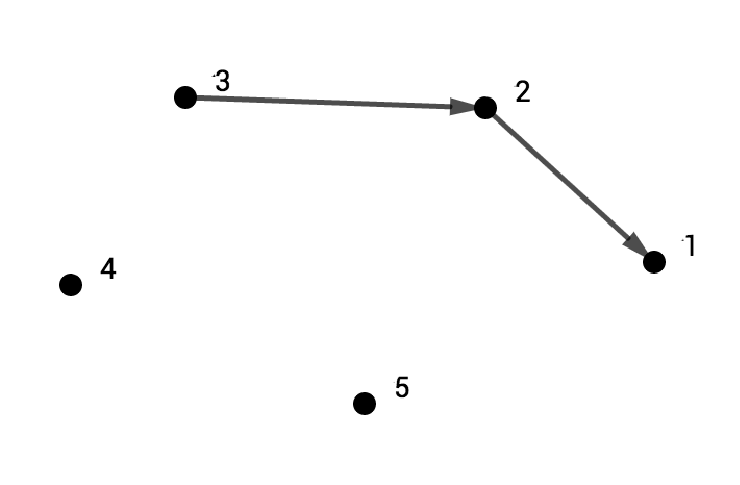
\includegraphics[width=4.5cm]{graph2.eps}
	\vspace{-5pt}
	\caption{Representation of agents and their interactions using a graph $G(t)$}	
	\label{fig2b}\vspace{-15pt}
\end{figure}

The ad-hoc nature of human interactions is modeled by asynchronous updates. When an agent modifies its belief under the influence of its neighbors ($\langle \theta_{i}(t)\rangle$), it is governed by 
\begin{align}\label{e1}
\begin{split}
&\theta_{i}(t+1) = \langle \theta_{i}(t)\rangle,\\ 
& \tan(\langle \theta_{i}(t)\rangle)=\frac{\sum\limits_{j\in N_{D_{i}}(t)\cup \bar{N}_{ND_{i}}(t)} w_{ij}(t) \sin(\theta_{j}(t))}{ \sum\limits_{j\in N_{D_{i}}(t)\cup \bar{N}_{ND_{i}}(t)}w_{ij}(t) \cos(\theta_{j}(t))}.
\end{split}
\end{align}
Whenever agents interact and update their beliefs, the network topology may change; the updated belief of an agent may impact its neighborhood set, and thereby, the network's edges. 


The edges are classified as direct and non-direct ties. Direct ties are an agent's frequent contacts belonging to $N_{D_{i}}(t)$, and are its one-hop neighbors. Non-direct ties are occasional contacts belonging to $N_{ND_i}(t)$, and are an agent's two-hop or three-hop neighbors, such that,
\begin{equation}
N_{i}(t) = N_{D_{i}}(t)\cup N_{ND_{i}}(t).
\end{equation} 
This is essential because, like-minded agents may be unaware of each others' presence in a vast network. When an agent updates its belief using (\ref{e1}), it considers $N_{D_{i}}(t)$ and a randomly chosen subset, $\bar{N}_{ND_{i}}(t) \subseteq N_{ND_{i}}(t)$. This way, noise is inherent in our model; greater an agent's tolerance, more susceptible it is to such chanced interactions.

Trust scores - $w_{ij}(t),~\text{with}~j~\neq~i$, in (\ref{e1}) associated with edges signify the strength of an influence. Initially, direct ties are assigned random trust scores ($w_{ij}(t)$). Between a pair of vertices $(j,i)$, a sequence of directed edges connecting them is a directed path. To compute the weight of a non-direct tie, all such paths between the vertex pair are identified. The weight of each path is defined as the product of weights of the edges that constitute them. The score of a temporary edge is the average of the weights of all such paths between a pair $(j,i)$;
\begin{align}
\begin{split}
&w_{ij}(t)=\frac{\sum\limits_{p=1}^{p_{max}}\prod\limits_{(m,n)\in E_{path}}w_{mn}(t)}{p_{max}},\\
&E_{path}=\{(m,n)|\ (m,n)\in \text{the directed path}~ (j,i) \},\\
&p_{max}=|E_{path}|,~\sum_{j,j\neq i}w_{ij}(t)~=~ 1-w_{ii}(t).
\end{split}
\end{align}
Hence, the influences of direct ties are stronger. Evidently, the trust scores are proposed based on familiarity of agents - frequent or occasional contact.

The self-weights ($w_{ii}(t)$) reflect an agent's status in the network. To measure them, we use Katz's centrality, 
\begin{equation}
W(t)~=~\beta(I-\alpha A^{T}(t))^{-1}~.~\mathbf{1},
\end{equation} 
where, $\beta$ is a positive non-zero bias, $\alpha <1/\lambda_{max}$, $A(t)$ is the adjacency matrix of the underlying network, and $W(t)$ is a vector of self-weights. Accordingly, the importance of a node is based not only on its degree, but also on the nature of its contacts. Essentially, a node's connection to influential nodes yields a higher self-weight than ties with less prominent ones. Additionally, a socially important individual is less obligated to yield to influence, which is reflected in (\ref{e1}), where, self-weights quantify the importance accorded to one's opinion. 

Upon interactions, new connections are forged only with non-direct ties, since, humans do not reach-out beyond them \cite{christakis2009connected}. A new tie is gained when the cumulative number of random interactions between agent $i$ and its non-direct tie $j$, exceeds its sociability index ($s_{i}$). Under the assumption that socially important agents do not forge ties easily, the index is assumed to be proportional to self-weight;
\begin{equation}
s_{i} = K_{C}w_{ii},
\end{equation}
where, $K_{C}$ is a proportionality constant, chosen based on the network size. Also, it has been observed that inter-personal bonds are not easily lost. Therefore, only the ties between agents with dissimilar opinions disappear; agent $i$ loses a direct tie $j$ when the following condition is violated, 
\begin{equation}
|\theta_{i}(t)-\theta_{j}(t)|\leq\theta_{T_{i}}.
\end{equation}

\section{PROBLEM FORMULATION}
Consider $N$ agents, each with a belief $\theta_{i}(t)$ and a tolerance $ \theta_{T_{i}}$. The beliefs are updated using (\ref{e1}), and the interactions are governed by rules prescribed in the previous section. As beliefs change, the underlying network topology evolves. This interplay yields different collective behaviors. We are interested in studying consensus or the lack of it, subject to different (1) initial opinion spreads, (2) constituent agent types, (3) individual tolerance, and (4) densities of agents. The agents could be rigid or flexible based on their individual tolerance. The groups they constitute could either be liberal or conservative based on their collective opinion spread. 

\subsection{Classification of Agents}
The agents are grouped based on their tolerances;
\begin{enumerate}
	\item{Rigid:} They are stubborn individuals that interact with similar agents. Their intolerance to diverse beliefs is modelled with lower thresholds, $\theta_{T_{i}}\in[0,\theta_{R}]$.
	
	\item{Flexible:} They admit beliefs very different from their own, and are modelled with high tolerances, $\theta_{T_{i}}\in[\theta_{F_{1}},\theta_{F_{2}}]$, such that, $\theta_{F_{2}}>\theta_{F_{1}}>\theta_{R}$.  
\end{enumerate}
In this work, fixed tolerances of rigid or flexible individuals does not necessarily translate to interactions between all similar-minded individuals due to the familiarity-based distinction. 


\subsection{Classification of Groups}

The groups are classified depending on the initial distribution of their agents' beliefs. In real, opinions may not be uniformly spread.  Instead, there could be a popular opinion with deviations. Therefore, we employ a truncated Gaussian model whose mean ($\mu$) and standard deviation ($\sigma$) represent the popular opinion and the nature of the group, respectively. Accordingly, the groups are classified as,
\begin{enumerate}
	\item{Conservative:} The agents' initial beliefs are typically in the vicinity of a popular opinion ($\mu$), as such groups allow only a few contrarians (in Fig. \ref{fig5b}). This is modelled using a small spread $\sigma \in [0,\theta_{C}]$.
	\item{Liberal:} It admits varied opinions, and this diversity is reflected in a larger spread, $\sigma \in [\theta_{L_{1}},\theta_{L_{2}}]$, where, $\theta_{L_{2}}>\theta_{L_{1}}>\theta_{C}$ (in Fig. \ref{fig5d}).
	\begin{figure}
		\subfigure[PDF of a conservative group]{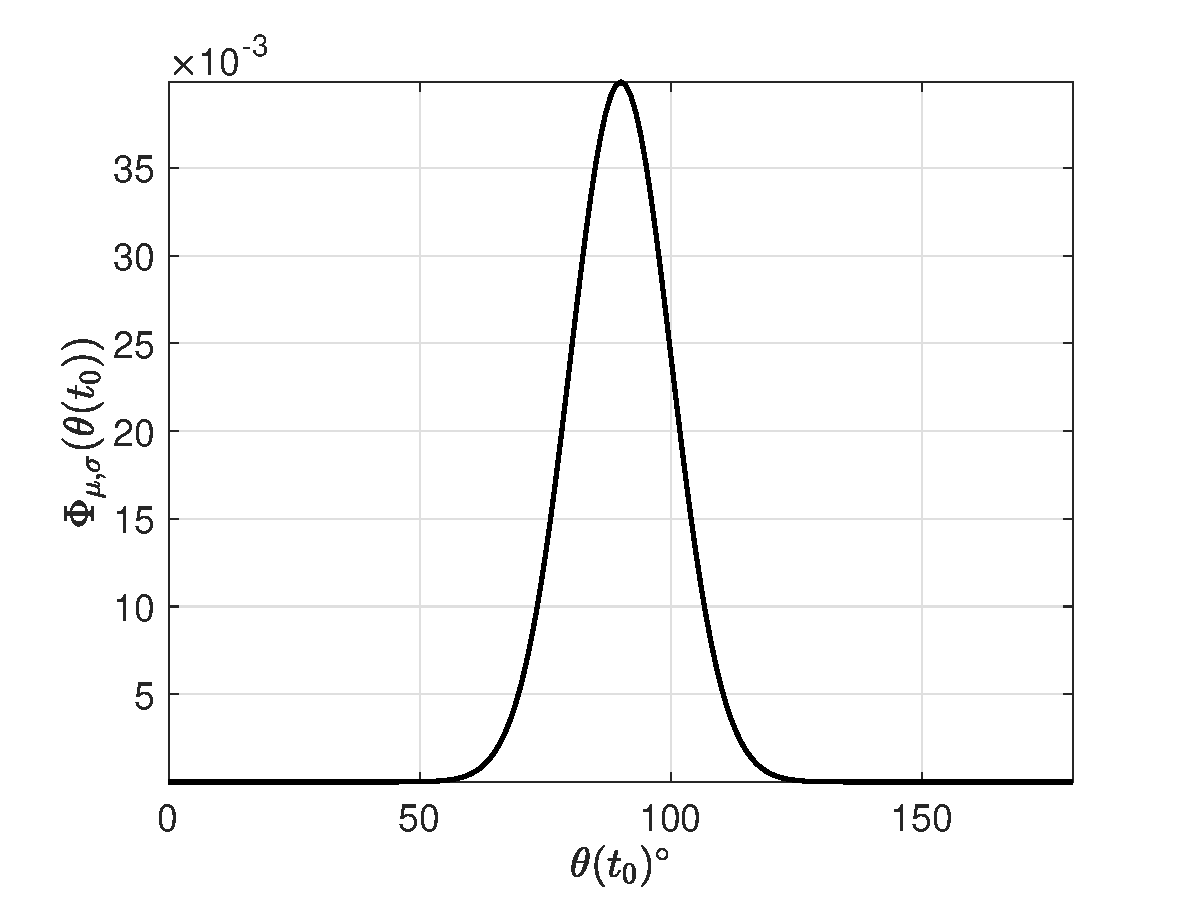
\includegraphics[width=4.cm]{conservativepdf.eps}
			\label{fig5a}}
		\hfil
		\subfigure[Opinions in a conservative group]{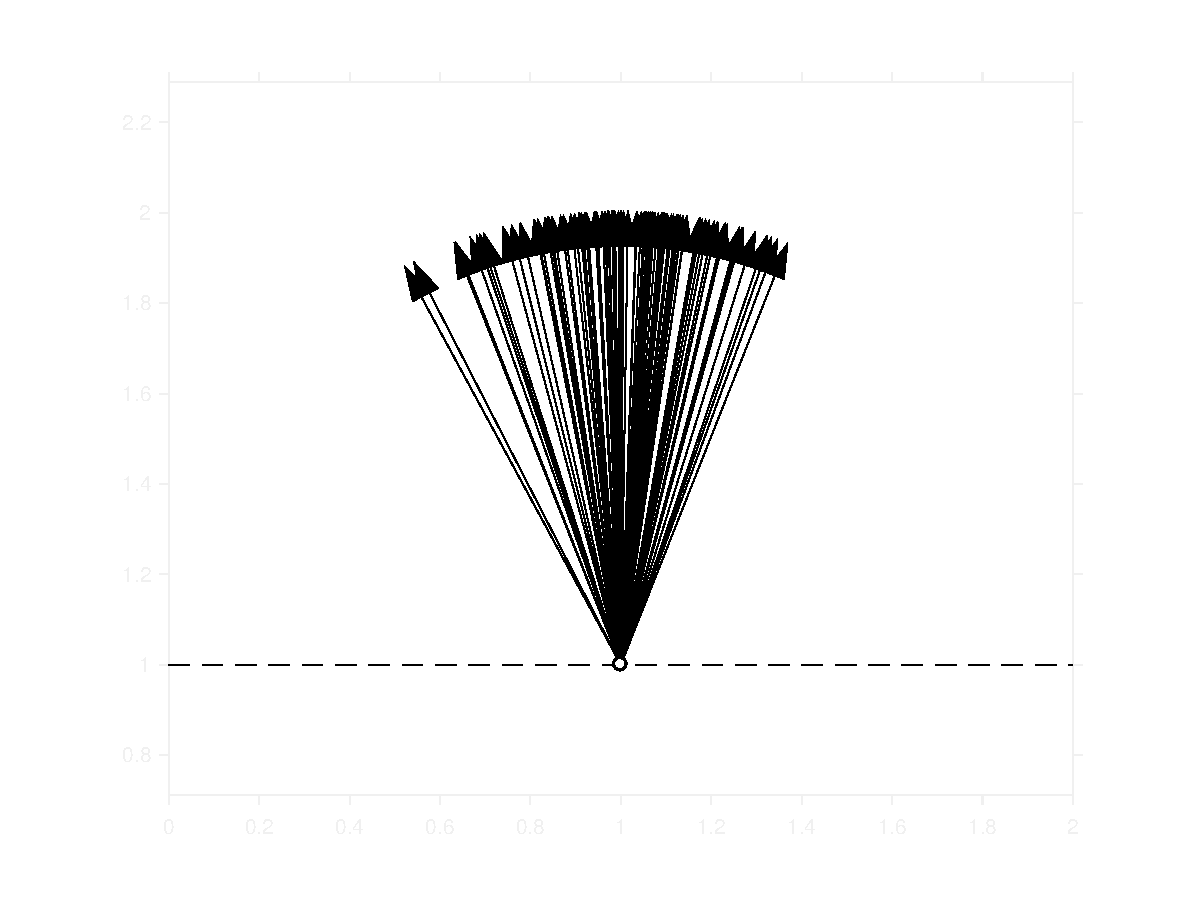
\includegraphics[width=4.cm]{conservativeopinions.eps}\label{fig5b}}
		\subfigure[PDF of a liberal group]{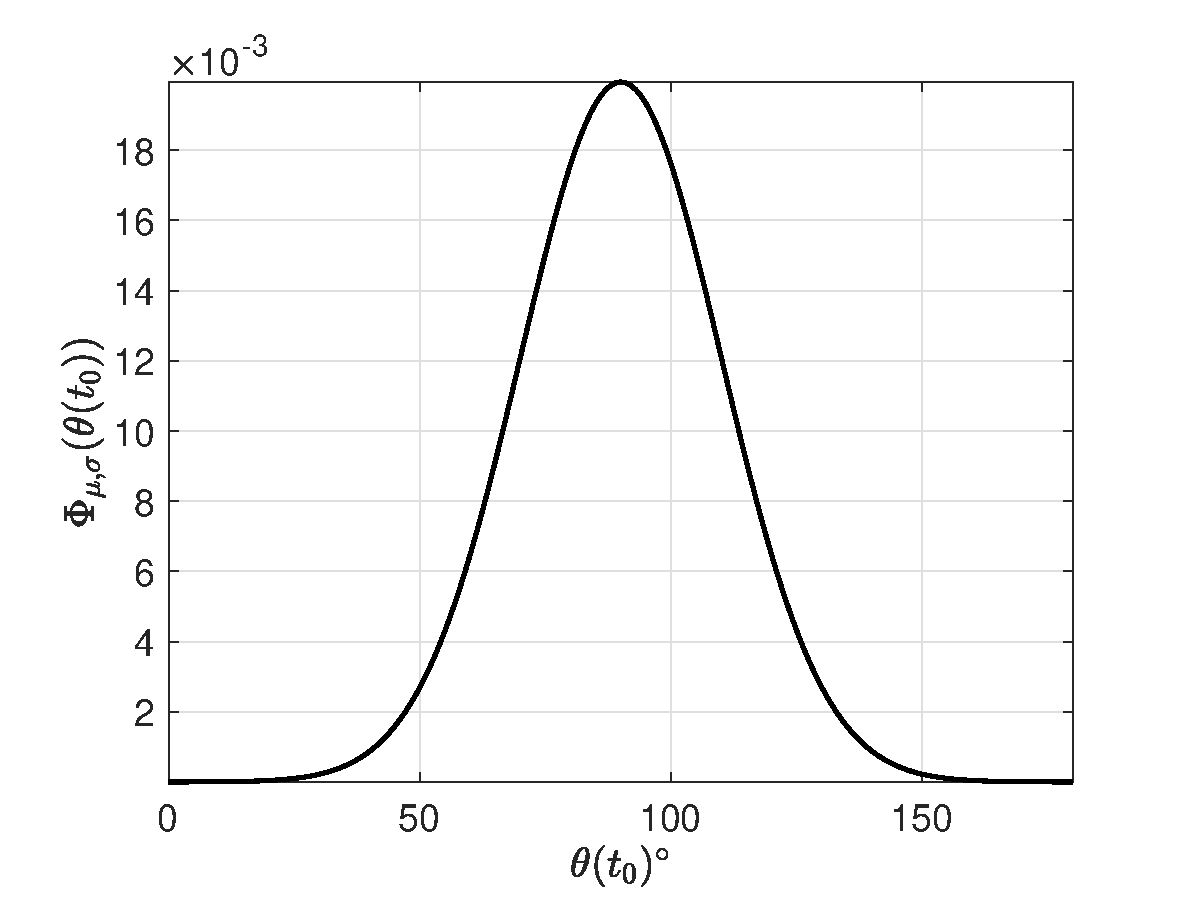
\includegraphics[width=4.cm]{liberalpdf.eps}\label{fig5c}}
		\hfil
		\subfigure[Opinions in a liberal group]{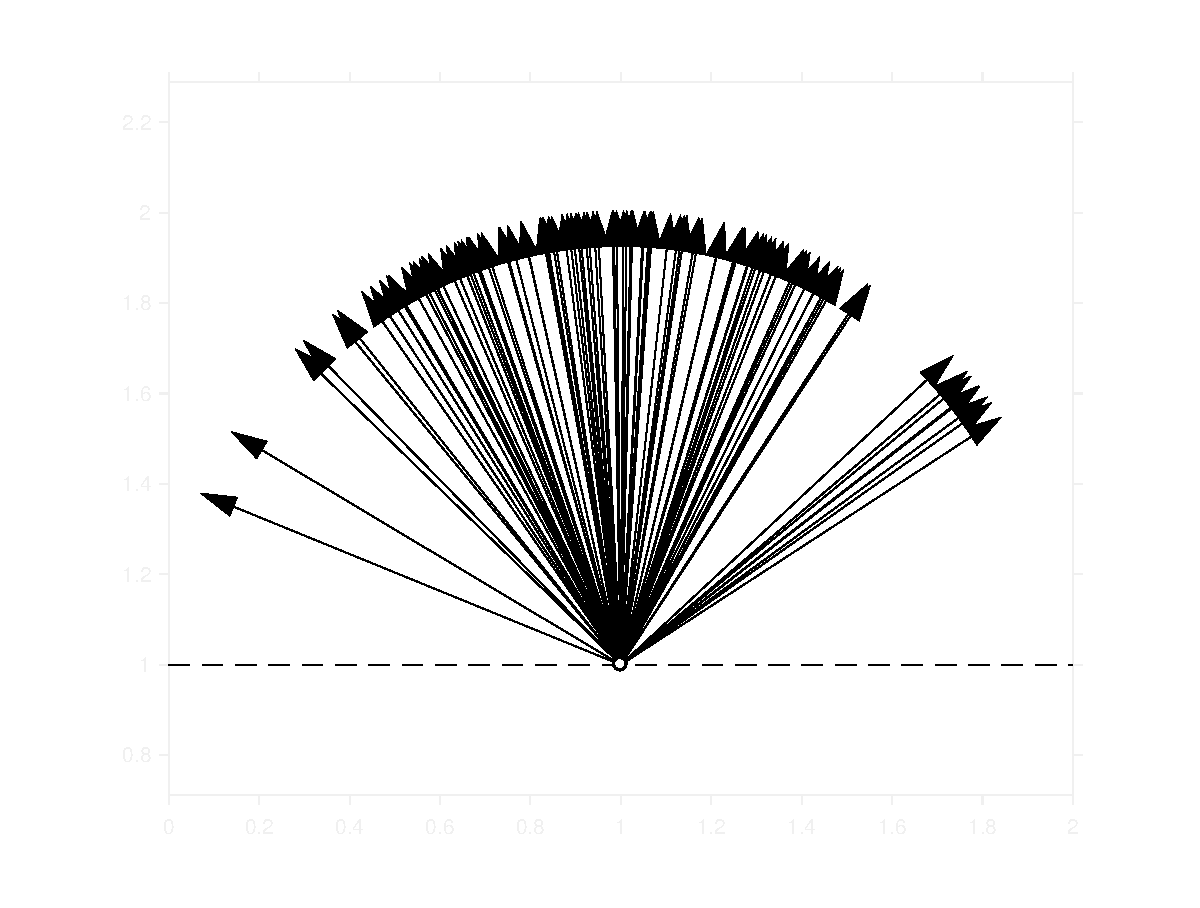
\includegraphics[width=4.cm]{liberalopinions.eps}\label{fig5d}}
		\caption{Truncated Gaussian distribution of initial opinions}
		\label{fig5}
	\end{figure}
\end{enumerate}

\section{SIMULATION RESULTS \& DISCUSSIONS}

A group of 100 agents has been considered with the simulation time set at 250 units. For instance, all rigid agents have a tolerance $\theta_{R} \in \{10^\circ,30^\circ\}$, while all flexible agents have a tolerance $\theta_{F} \in \{40^\circ,80^\circ\}$. The distribution of initial opinions for conservative and liberal groups are set at $\mu = 90^\circ$ with $\sigma \in \{10^\circ,15^\circ\}$ and $\sigma \in \{20^\circ,25^\circ\}$, respectively. The initial network is derived from opinions and tolerances. There are no assumptions made regarding the structure of the initial network. To prevent trivial initial networks - like well-connected ones - the out-degree of each vertex is capped at 25. The constant of proportionality, $K_{C}$, is set to 100. To account for diverse opinions, network topologies, and interaction patterns, Monte Carlo simulations have been carried out.	

To this end, we define four group configurations,

\begin{enumerate}
	\item Configuration 1 is a conservative group with all rigid agents, or more rigid agents than flexible ones.
	\item Configuration 2 is a conservative group with all flexible agents, or more flexible agents than rigid ones.
	\item Configuration 3 is a liberal group, where, the density of agents is similar to Configuration 1.
	\item Configuration 4 is also a liberal group, where, the density of agents is similar to Configuration 2.
	
\end{enumerate}
 Each configuration with fixed agent tolerances is subjected to 100 simulation runs. Each run corresponds to a particular opinion distribution, fixed agents' density and tolerance -            $\{10^\circ,30^\circ,40^\circ\,80^\circ\}$. Starting with a group of all flexible agents, we study the impact of density of rigid agents on consensus. This is quantified by, 
\begin{align}
\small
\begin{split}
&\text{Rate of Consensus} = \frac{\text{ No. of times group consensus is achieved}}{\text{No. of simulation trials}}.
\end{split}
\end{align}
 The consensus rate for a configuration is essentially the average occurrence of group consensus.
 \begin{figure*}
 	\centering
 	\subfigure[Conservative group with $\sigma = 10^{\circ}$]{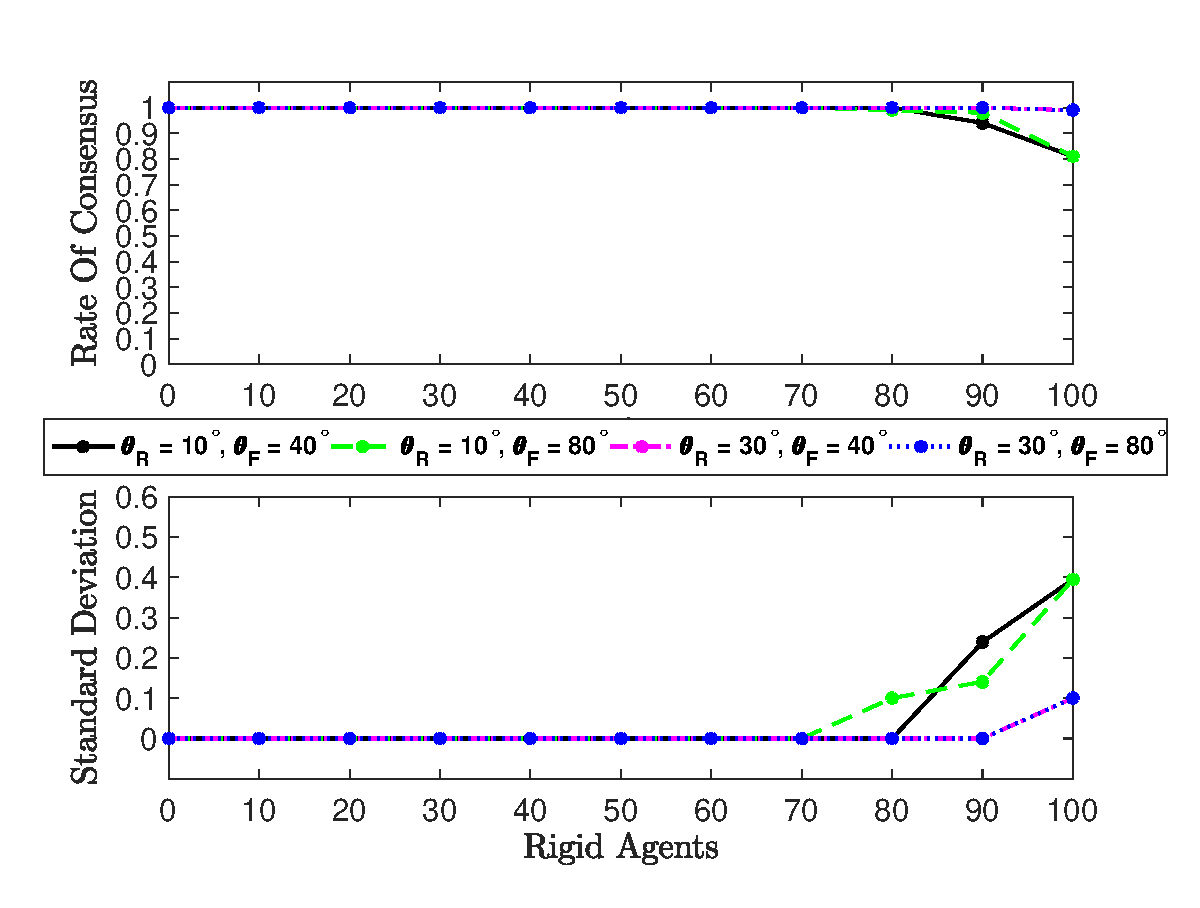
\includegraphics[width=0.45\textwidth]{conservative1.eps}
 		\label{fig6a}}
 	\hfil
 	\subfigure[Conservative group with $\sigma = 15^{\circ}$]{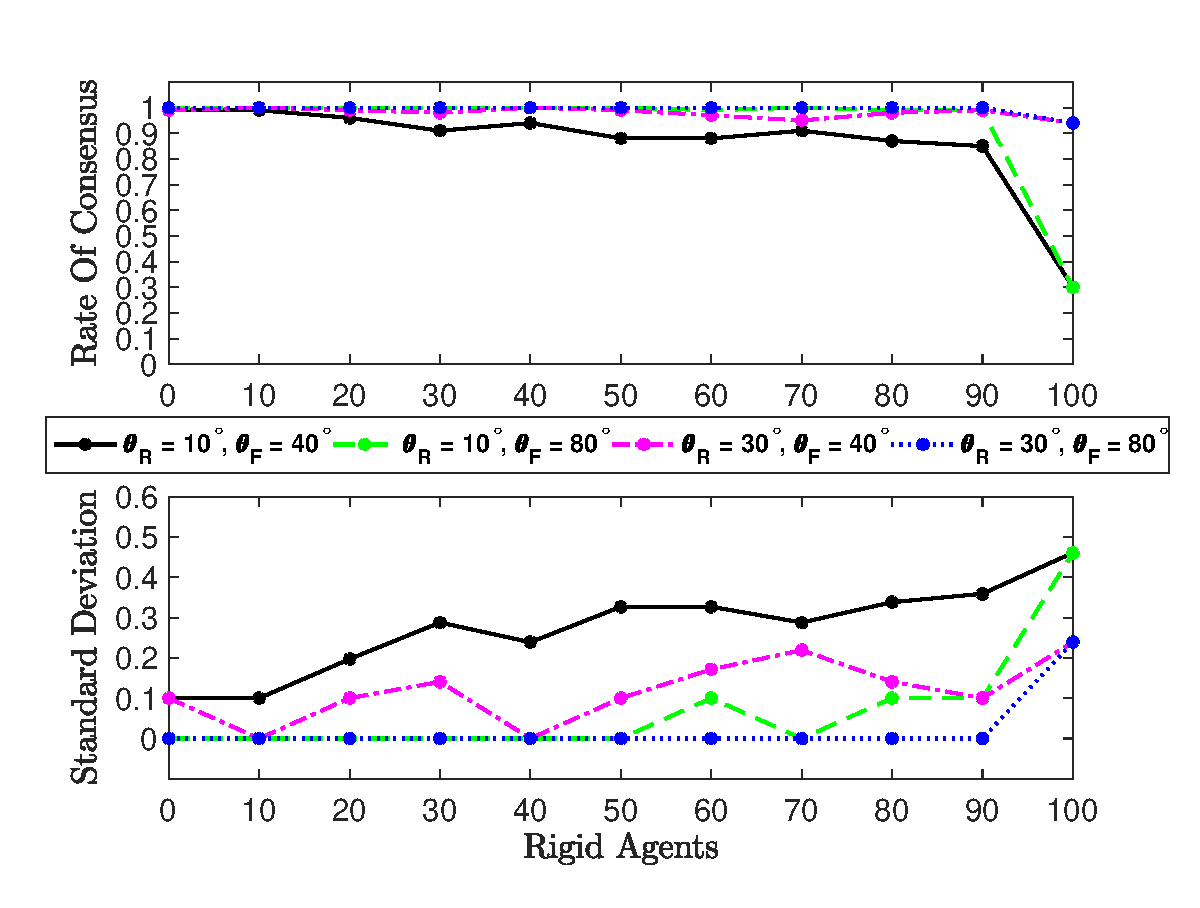
\includegraphics[width=0.45\textwidth]{conservative2.eps}
 		\label{fig6b}}
 	\hfil
 	\subfigure[Liberal group with $\sigma = 20^{\circ}$]{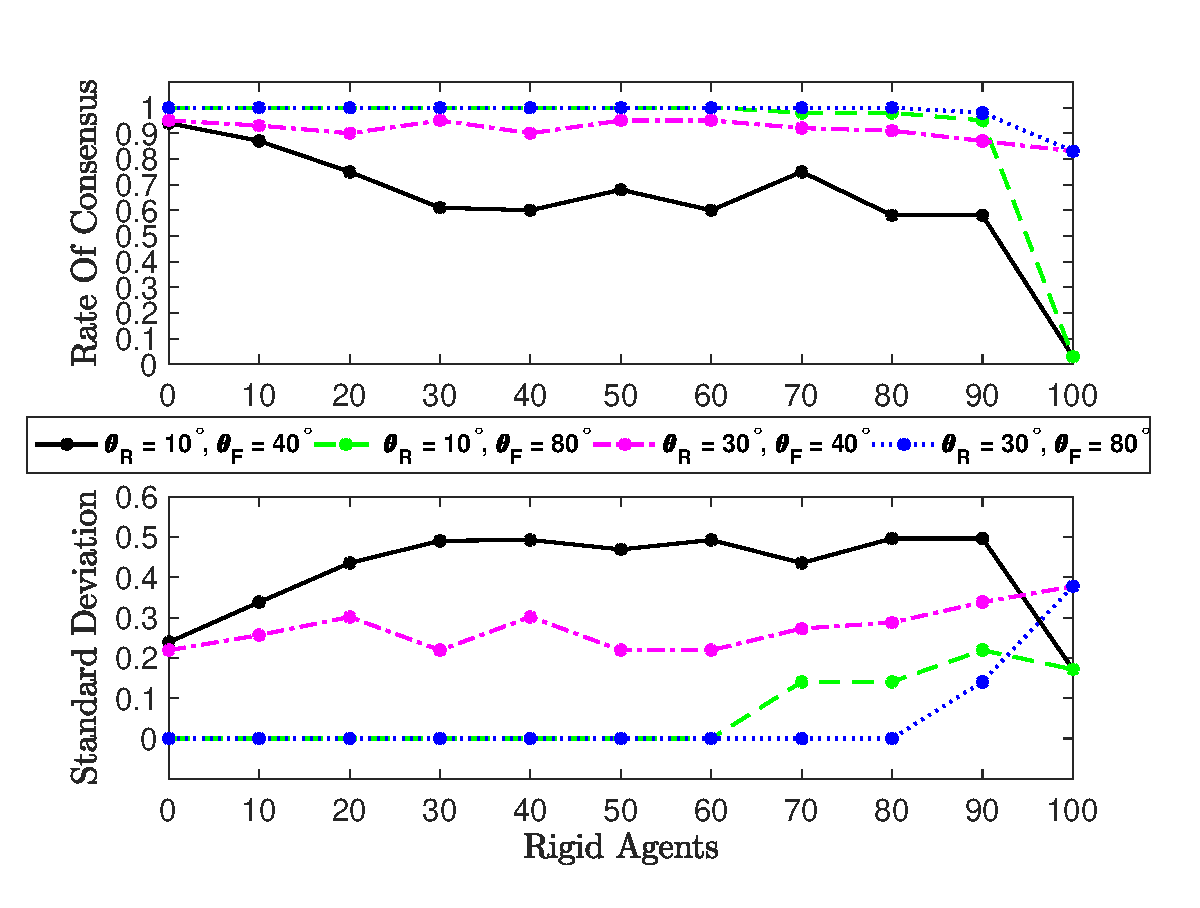
\includegraphics[width=0.45\textwidth]{liberal1.eps}\label{fig6c}}
 	\hfil
 	\subfigure[Liberal group with $\sigma = 25^{\circ}$]{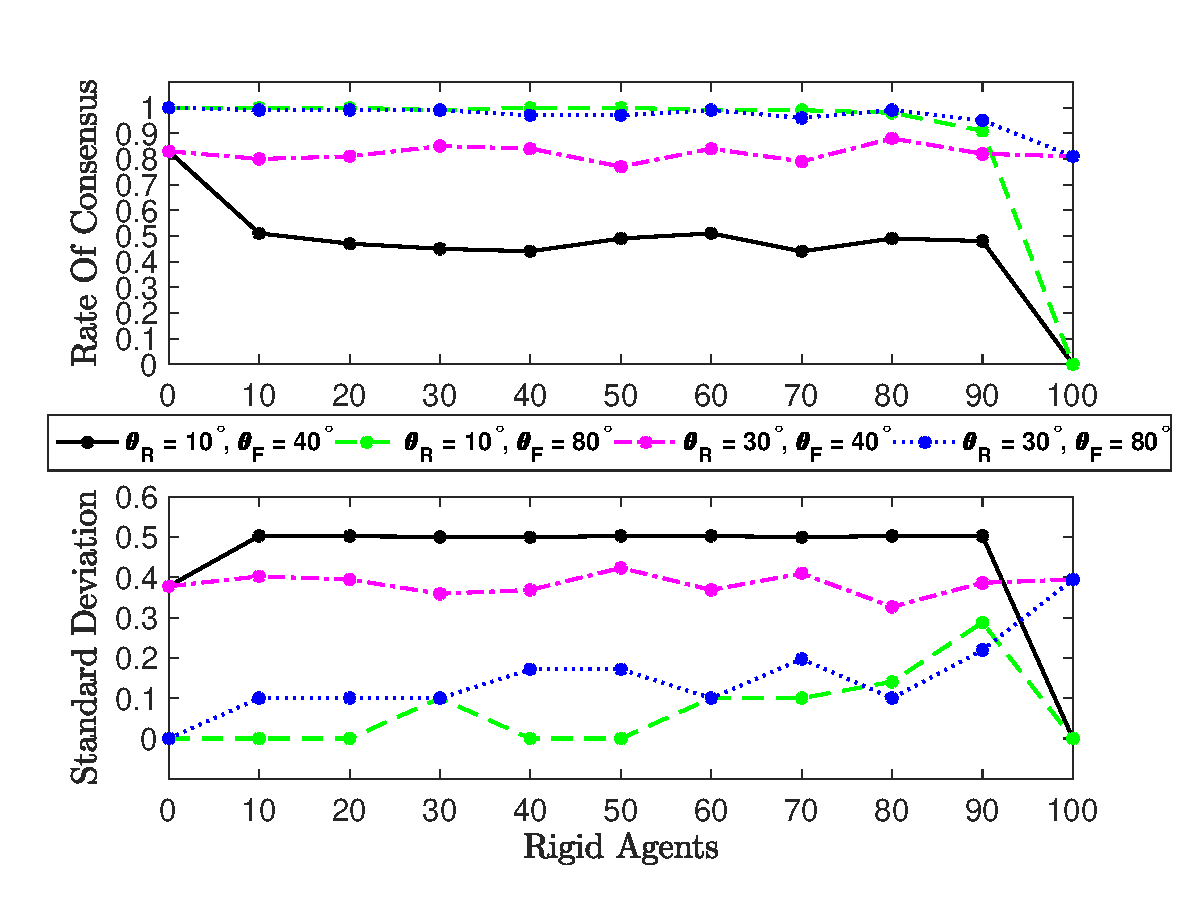
\includegraphics[width=0.45\textwidth]{liberal2.eps}\label{fig6d}}
 	\caption{Rate of consensus in conservative and liberal groups with varying agent densities and individual tolerance}
 	\label{fig6}
 \end{figure*}

In conservative groups, when flexible agents are in a majority, the dialogue between agents mostly yields consensus. On increasing the number of rigid members in the group, factions are formed. This is captured by a marginal drop in the consensus rate in Fig. \ref{fig6a} and Fig. \ref{fig6b}. 
 
 In liberal groups, the rate of consensus is impacted not only by rigid agents, but also by a wider initial belief distribution. Intuitively, a group with all flexible individuals should have a relatively high rate of consensus for different values of $\theta_{T_{i}}$ and different initial spreads, which is also observed in Fig. \ref{fig6}. However, with increase in the population of rigid agents in an all flexible group, there is a significant drop in the rate of consensus (see Fig. \ref{fig6c} and Fig. \ref{fig6d}).
 
 \section{CONCLUSIONS}
 We discussed a modified Vicsek-like model to study influence dynamics, its spread and consequence on opinions. The heading angles of agents in \cite{vicsek1995novel} are considered analogous to beliefs, while ignoring their physical distances. A closest-opinion rule with a familiarity-based distinction has been proposed which is equipped to handle the subtleties in human interactions, and opinion formation. To emulate real-life scenarios, we have considered different agent types, groups, and their compositions. In addition to confirming anticipated behaviour, the results are in sync with similar reports in literature. 
 
\begin{thebibliography}{99}
	\bibitem{vicsek1995novel} Vicsek, T., Czirók, A., Ben-Jacob, E., Cohen, I., \& Shochet, O. (1995). Novel type of phase transition in a system of self-driven particles. Physical review letters, 75(6), 1226.
	\bibitem{2} Vedam, N., \& Ghose, D. (2018). Influence Dynamics and Consensus in an Opinion-Neighborhood based Modified Vicsek-like Social Network. arXiv preprint arXiv:1808.10716.
	\end{thebibliography}
\end{document}
